\documentclass{standalone}
\usepackage{tikz}
\usepackage{verbatim}
\begin{document}
\pagestyle{empty}
  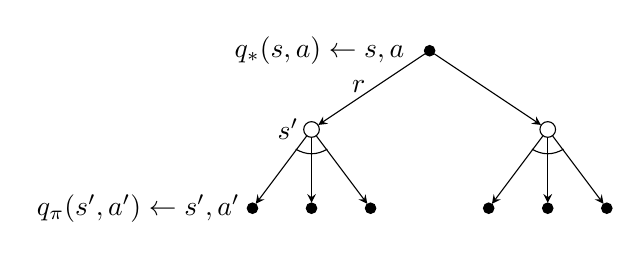
\begin{tikzpicture}
    \node[draw,circle, fill, scale=0.4] (s) at (0,0) {};
    \node at (-1.4, 0) {$q_{*}(s,a) \leftarrow s, a$};
    \foreach \x in {-1, 1} {
      \node[draw,circle,scale=0.6] (b\x) at (1.5*\x, -1) {};
      \draw[-stealth] (s) -- (b\x);
      
      \node[draw,circle,fill, scale=0.4] (l\x) at (1.5*\x-.75,-2) {};
      \node[draw,circle,fill, scale=0.4] (m\x) at (1.5*\x,-2) {};
      \node[draw,circle,fill, scale=0.4] (r\x) at (1.5*\x+.75,-2) {};
      \draw[-stealth] (b\x) -- (l\x);
      \draw[-stealth] (b\x) -- (m\x);
      \draw[-stealth] (b\x) -- (r\x);
    }
    \node at (-1.8, -1) {$s'$};
    \node at (-0.9, -0.45) {$r$};
    \node at (-3.7, -2) {$q_{\pi}(s',a') \leftarrow s', a'$};
    \path[-] (-1.7,-1.25) edge[bend right=30] (-1.3, -1.25);
    \path[-] (1.3,-1.25) edge[bend right=30] (1.7, -1.25);
  \end{tikzpicture}
\end{document}